\documentclass[12pt,a4paper]{article}

\usepackage{amsmath}
\usepackage{amssymb}
\usepackage{geometry}
\geometry{margin=2.5cm}
\usepackage{booktabs}
\usepackage{xcolor}
\usepackage{hyperref}
\usepackage{listings}
\usepackage{pgfplots}
\pgfplotsset{compat=1.18}
\usepackage{tcolorbox}
\tcbuselibrary{skins, breakable}
\usepackage{enumitem}
\usepackage{fancyhdr}
\usepackage{tikz}
\usepackage{array}

\newtcolorbox{curiositybox}[1]{colback=yellow!10, colframe=orange!80!black, fonttitle=\bfseries, title=#1, breakable}
\newtcolorbox{infobox}[1]{colback=blue!5, colframe=blue!60!black, fonttitle=\bfseries, title=#1, breakable}
\newtcolorbox{mistakebox}[1]{colback=red!5, colframe=red!60!black, fonttitle=\bfseries, title=#1, breakable}
\newtcolorbox{learnbox}[1]{colback=green!5, colframe=green!60!black, fonttitle=\bfseries, title=#1, breakable}

\lstset{language=Python, basicstyle=\ttfamily\small, keywordstyle=\color{blue},
        commentstyle=\color{gray}, stringstyle=\color{orange},
        showstringspaces=false, numbers=left, numberstyle=\tiny,
        breaklines=true, frame=single}

\pagestyle{fancy}
\fancyhf{}
\lhead{Topic 06: Fourier Integral Theorem}
\rhead{Unit V --- Fourier Series \& Transforms}
\cfoot{\thepage}

\title{Topic 06: Fourier Integral Theorem, Sine \& Cosine Integrals, Complex Form \\
\large Unit V --- Fourier Series \& Fourier Transforms}
\author{23A54201 --- Mathematics IV (Transform Techniques) \\
JNTUA College of Engineering (Autonomous)}
\date{}

\begin{document}
\maketitle
\tableofcontents
\newpage

%% ============================================================
\section{Opening Hook}
%% ============================================================

\begin{curiositybox}{Hook}
Fourier series works beautifully for periodic signals. But a single pulse of voltage that fires once and never repeats --- like a radar ping or a door-slam --- is not periodic at all. Its period is effectively infinite. What happens to the Fourier series when we let $L \to \infty$? The sum over discrete harmonics $n$ becomes an integral over a continuous frequency variable $\lambda$. This passage from sum to integral is the Fourier Integral Theorem, and it unlocks the analysis of ALL signals, periodic or not.
\end{curiositybox}

%% ============================================================
\section{Why This Topic Exists}
%% ============================================================

Before we begin, here is the honest answer to why you are reading this: periodic functions are a very special case of all possible signals. Most real-world signals --- radar pulses, door-slams, transient electrical spikes, a single beat of a heart --- appear once and never exactly repeat. Fourier series, which requires periodicity, simply cannot handle these functions in its standard form. We need a continuous-frequency representation, and the Fourier Integral Theorem provides exactly that.

The table below shows what goes wrong when you try to work without this theorem:

\begin{center}
\begin{tabular}{>{\bfseries}p{0.42\textwidth} p{0.48\textwidth}}
\toprule
\textbf{Mistake} & \textbf{Consequence} \\
\midrule
Trying to apply Fourier series to a non-periodic function & Getting no valid result at all --- the formulas produce meaningless coefficients \\
\midrule
Skipping the limiting argument ($L\to\infty$) & Not understanding where the Fourier integral formula comes from; memorising a formula without comprehension \\
\midrule
Confusing Fourier integral with Fourier transform & Treating them as unrelated formulas when the transform is simply a compact notation for the integral \\
\bottomrule
\end{tabular}
\end{center}

\begin{learnbox}{What You Need to Remember from This Section}
The Fourier Integral Theorem is the bridge from the periodic world (Fourier series, discrete harmonics) to the non-periodic world (continuous frequency spectrum). Every concept in this topic is a natural extension of what you already know.
\end{learnbox}

%% ============================================================
\section{You Already Know This (Intuition First)}
%% ============================================================

Think of the frequency axis as a number line. In a Fourier series with half-period $L$, the harmonics live at the discrete points $0,\, \frac{1}{L},\, \frac{2}{L},\, \frac{3}{L}, \ldots$ on that line --- like the teeth of a comb, spaced $\frac{1}{L}$ apart. Each tooth carries an amplitude coefficient $a_n$ or $b_n$.

Now imagine slowly inflating the period: $L = 10$, then $100$, then $10000$, then $\infty$. The comb teeth get closer and closer together: $\frac{1}{10},\, \frac{1}{100},\, \frac{1}{10000}, \ldots$ All the way down to zero spacing. At that limit, the discrete comb of harmonics becomes a continuous curve --- a function of $\lambda$. The sum $\sum_n (\cdots)\frac{1}{L}$ becomes a Riemann integral $\int_0^\infty (\cdots)\,d\lambda$.

This is exactly the same logic by which a finite sum $\sum_{k=1}^N f(x_k)\Delta x$ becomes the definite integral $\int_a^b f(x)\,dx$ when you let $N\to\infty$ and $\Delta x\to 0$. Nothing new --- just the familiar passage from discrete to continuous.

%% ============================================================
\section{The Fourier Integral Theorem (Statement Without Proof)}
%% ============================================================

\begin{infobox}{Fourier Integral Theorem}
Let $f(x)$ be a function defined on $(-\infty,\infty)$ such that:
\begin{itemize}
  \item $f(x)$ is \textbf{absolutely integrable}: $\displaystyle\int_{-\infty}^{\infty}|f(x)|\,dx < \infty$
  \item $f(x)$ is \textbf{piecewise smooth} on every finite interval
\end{itemize}
Then at every point where $f$ is continuous:
\[
  f(x) = \int_0^\infty \Bigl[A(\lambda)\cos(\lambda x) + B(\lambda)\sin(\lambda x)\Bigr]\,d\lambda
\]
where the \textbf{Fourier integral coefficients} are:
\[
  A(\lambda) = \frac{1}{\pi}\int_{-\infty}^{\infty} f(t)\cos(\lambda t)\,dt, \qquad
  B(\lambda) = \frac{1}{\pi}\int_{-\infty}^{\infty} f(t)\sin(\lambda t)\,dt
\]
At a jump discontinuity $x_0$, the integral converges to the average value $\dfrac{f(x_0^+)+f(x_0^-)}{2}$.

\textit{Note:} Formal proof (via the $L\to\infty$ passage) is not required for this course. The intuition is given in Section 3.
\end{infobox}

Physically, $A(\lambda)$ measures \textit{how much cosine of frequency $\lambda$} is present in $f$, and $B(\lambda)$ measures \textit{how much sine}. Together they build up the complete spectral picture of any absolutely integrable signal.

%% ============================================================
\section{Fourier Cosine Integral (for Even Functions)}
%% ============================================================

\begin{infobox}{Fourier Cosine Integral}
If $f(x)$ is an \textbf{even} function on $(-\infty,\infty)$ --- meaning $f(-x)=f(x)$ --- or if $f$ is defined only on $(0,\infty)$ and we extend it evenly, then $f(t)\sin(\lambda t)$ is odd in $t$ and so its integral over $(-\infty,\infty)$ vanishes: $B(\lambda)=0$. The representation simplifies to:
\[
  f(x) = \frac{2}{\pi}\int_0^\infty A_c(\lambda)\cos(\lambda x)\,d\lambda
\]
where the \textbf{Fourier cosine transform} of $f$ is:
\[
  A_c(\lambda) = \int_0^\infty f(t)\cos(\lambda t)\,dt
\]
This is more convenient than the full integral whenever the function has even symmetry.
\end{infobox}

Note the factor: the full theorem has $\frac{1}{\pi}$ in $A(\lambda)$ and integrates over $(-\infty,\infty)$. The cosine integral absorbs the factor of $2$ (from symmetry) and restricts to $(0,\infty)$, giving $A_c(\lambda) = \pi A(\lambda)/2 \cdot 2/\pi \cdot \pi$ --- matching to $\frac{2}{\pi}\int_0^\infty A_c(\lambda)\cos(\lambda x)\,d\lambda$. Keep the formulas as stated; do not mix the two conventions.

%% ============================================================
\section{Fourier Sine Integral (for Odd Functions)}
%% ============================================================

\begin{infobox}{Fourier Sine Integral}
If $f(x)$ is an \textbf{odd} function on $(-\infty,\infty)$ --- meaning $f(-x)=-f(x)$ --- or if $f$ is defined only on $(0,\infty)$ and we extend it oddly, then $f(t)\cos(\lambda t)$ is odd in $t$ and so $A(\lambda)=0$. The representation becomes:
\[
  f(x) = \frac{2}{\pi}\int_0^\infty B_s(\lambda)\sin(\lambda x)\,d\lambda
\]
where the \textbf{Fourier sine transform} of $f$ is:
\[
  B_s(\lambda) = \int_0^\infty f(t)\sin(\lambda t)\,dt
\]
\end{infobox}

The practical rule: if a function is defined only on $(0,\infty)$ and you want to represent it as a half-range integral, you may \textit{choose} either the sine or the cosine integral by extending the function oddly or evenly respectively --- just as you chose half-range sine or cosine series in Topic 05.

%% ============================================================
\section{Complex Form of the Fourier Integral}
%% ============================================================

\begin{infobox}{Complex Form}
Using Euler's identity $e^{i\lambda x} = \cos(\lambda x) + i\sin(\lambda x)$ to combine the $A(\lambda)$ and $B(\lambda)$ integrals, the Fourier integral theorem can be written in the elegant complex form:
\[
  f(x) = \frac{1}{2\pi}\int_{-\infty}^{\infty}\left[\int_{-\infty}^{\infty}f(t)\,e^{-i\lambda t}\,dt\right]e^{i\lambda x}\,d\lambda
\]
The \textbf{inner bracket} is the \textbf{Fourier Transform} of $f$:
\[
  \mathcal{F}\{f(t)\} = F(\lambda) = \int_{-\infty}^{\infty} f(t)\,e^{-i\lambda t}\,dt
\]
The \textbf{outer integral} is the \textbf{Inverse Fourier Transform}:
\[
  f(x) = \frac{1}{2\pi}\int_{-\infty}^{\infty} F(\lambda)\,e^{i\lambda x}\,d\lambda
\]
So the complex Fourier integral theorem is simply the statement: \textit{the Fourier transform and its inverse are consistent}. This is precisely the topic of Topic 07 --- the complex form is the preview.
\end{infobox}

This reformulation does not add new information; it packages the real form into a cleaner notation that generalises naturally to complex-valued signals and to engineering conventions where complex exponentials are far easier to manipulate than separate sine and cosine integrals.

%% ============================================================
\section{Visualising Frequency Spectrum}
%% ============================================================

The figure below shows two panels for the rectangular pulse $f(x)=1$ for $|x|<1$, $f(x)=0$ otherwise. The top panel is the time-domain signal; the bottom panel shows its Fourier integral amplitude $A(\lambda) = \frac{2\sin\lambda}{\pi\lambda}$, which is the sinc function --- the prototypical frequency spectrum of a pulse.

\begin{center}
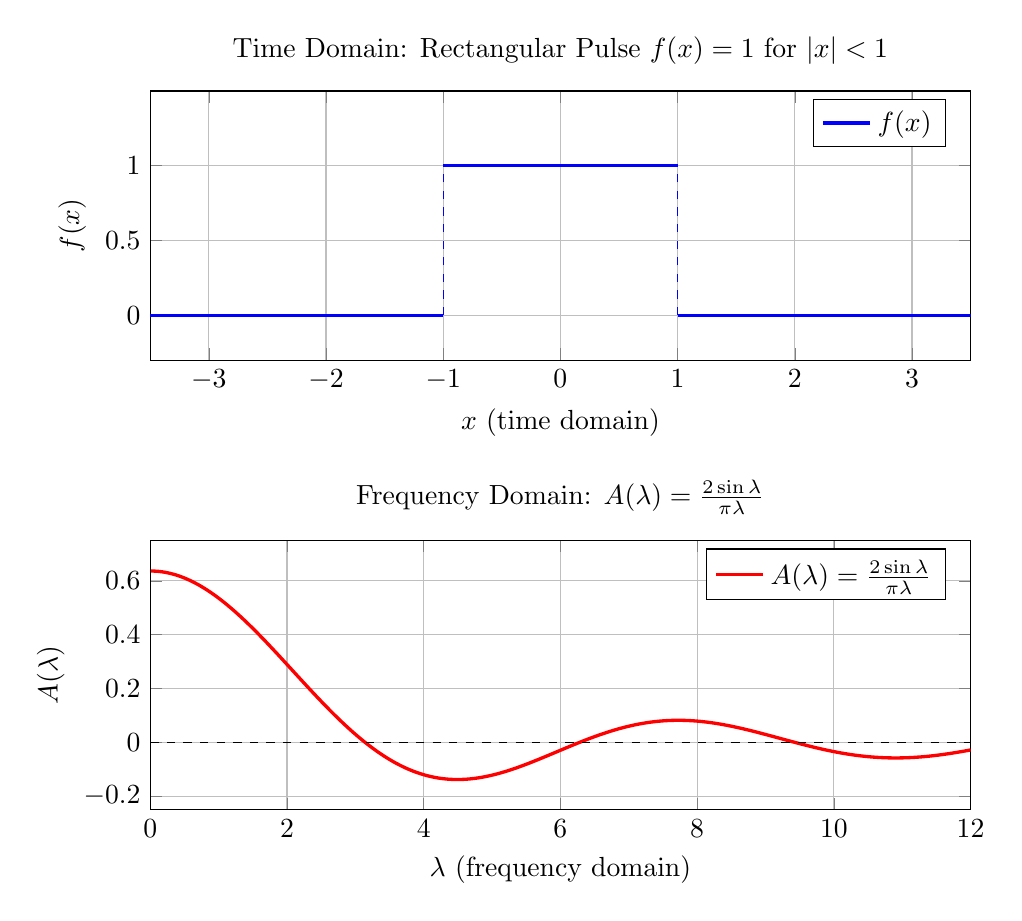
\begin{tikzpicture}
  % Top panel: time domain rectangular pulse
  \begin{axis}[
    name=timedomain,
    width=12cm, height=5cm,
    xlabel={$x$ (time domain)},
    ylabel={$f(x)$},
    xmin=-3.5, xmax=3.5,
    ymin=-0.3, ymax=1.5,
    grid=major,
    title={Time Domain: Rectangular Pulse $f(x)=1$ for $|x|<1$},
    xtick={-3,-2,-1,0,1,2,3},
    ytick={0,0.5,1},
    legend pos=north east
  ]
    \addplot[blue, very thick] coordinates {(-3.5,0)(-1,0)};
    \addplot[blue, very thick] coordinates {(-1,1)(1,1)};
    \addplot[blue, very thick] coordinates {(1,0)(3.5,0)};
    \addplot[blue, dashed] coordinates {(-1,0)(-1,1)};
    \addplot[blue, dashed] coordinates {(1,0)(1,1)};
    \addlegendentry{$f(x)$}
  \end{axis}
  % Bottom panel: frequency domain sinc
  \begin{axis}[
    at={(timedomain.below south west)}, anchor=north west,
    yshift=-1.2cm,
    width=12cm, height=5cm,
    xlabel={$\lambda$ (frequency domain)},
    ylabel={$A(\lambda)$},
    xmin=0, xmax=12,
    ymin=-0.25, ymax=0.75,
    grid=major,
    title={Frequency Domain: $A(\lambda)=\frac{2\sin\lambda}{\pi\lambda}$},
    legend pos=north east
  ]
    \addplot[red, very thick, domain=0.01:12, samples=300]
      {2*sin(deg(x))/(3.14159*x)};
    \addlegendentry{$A(\lambda)=\frac{2\sin\lambda}{\pi\lambda}$}
    \addplot[black, dashed] coordinates {(0,0)(12,0)};
  \end{axis}
\end{tikzpicture}
\end{center}

Observe that the main lobe of the sinc function is centred at $\lambda=0$ and the first zero crosses at $\lambda=\pi\approx3.14$. A narrower pulse would produce a wider main lobe --- this is the \textbf{time-bandwidth product} trade-off fundamental to signal processing.

%% ============================================================
\section{Worked Examples}
%% ============================================================

\begin{infobox}{Example 1 --- Fourier Integral of $f(x)=e^{-|x|}$}
\textbf{Problem:} Find the Fourier integral representation of $f(x)=e^{-|x|}$ and deduce the value of
$\displaystyle\int_0^\infty\frac{\cos(\lambda x)}{1+\lambda^2}\,d\lambda$.

\textbf{Step 1: Identify symmetry.}
Since $f(x)=e^{-|x|}$ satisfies $f(-x)=e^{-|-x|}=e^{-|x|}=f(x)$, the function is \textbf{even}.
Therefore $B(\lambda)=0$ and we use the cosine form.

\textbf{Step 2: Compute $A(\lambda)$.}
\begin{align*}
A(\lambda) &= \frac{1}{\pi}\int_{-\infty}^{\infty} e^{-|t|}\cos(\lambda t)\,dt \\
           &= \frac{2}{\pi}\int_0^{\infty} e^{-t}\cos(\lambda t)\,dt \quad \text{(using symmetry)}
\end{align*}
Use the standard result $\int_0^\infty e^{-at}\cos(\lambda t)\,dt = \dfrac{a}{a^2+\lambda^2}$ with $a=1$:
\[
A(\lambda) = \frac{2}{\pi}\cdot\frac{1}{1+\lambda^2}
\]

\textbf{Step 3: Write the Fourier integral representation.}
\[
e^{-|x|} = \int_0^\infty A(\lambda)\cos(\lambda x)\,d\lambda = \frac{2}{\pi}\int_0^\infty \frac{\cos(\lambda x)}{1+\lambda^2}\,d\lambda
\]

\textbf{Step 4: Deduce the definite integral.}
Rearranging:
\[
\int_0^\infty\frac{\cos(\lambda x)}{1+\lambda^2}\,d\lambda = \frac{\pi}{2}\,e^{-|x|}
\]
At $x=0$: $\displaystyle\int_0^\infty\frac{d\lambda}{1+\lambda^2} = \frac{\pi}{2}$, which matches $[\arctan\lambda]_0^\infty = \frac{\pi}{2}$. \checkmark
\end{infobox}

\begin{learnbox}{What Did We Learn? --- Example 1}
When $f$ is even, $B(\lambda)=0$ and we only need the cosine integral coefficient $A(\lambda)$. The key integral $\int_0^\infty e^{-at}\cos(\lambda t)\,dt = a/(a^2+\lambda^2)$ appears constantly in Fourier analysis; memorise it.
\end{learnbox}

\begin{infobox}{Example 2 --- Fourier Sine Integral of $f(x)=e^{-ax}$, $x>0$, $a>0$}
\textbf{Problem:} Find the Fourier sine integral representation of $f(x)=e^{-ax}$ for $x>0$, $a>0$.

\textbf{Step 1: Apply the sine integral formula.}
Since the problem asks for the sine integral, we extend $f$ oddly to $(-\infty,\infty)$ (or simply use the half-range formula directly):
\[
B_s(\lambda) = \int_0^\infty f(t)\sin(\lambda t)\,dt = \int_0^\infty e^{-at}\sin(\lambda t)\,dt
\]

\textbf{Step 2: Evaluate $B_s(\lambda)$ by parts.}
Let $I = \int_0^\infty e^{-at}\sin(\lambda t)\,dt$. Integrate by parts twice:
\begin{align*}
I &= \left[-\frac{e^{-at}}{a}\sin(\lambda t)\right]_0^\infty + \frac{\lambda}{a}\int_0^\infty e^{-at}\cos(\lambda t)\,dt \\
  &= 0 + \frac{\lambda}{a}\left(\left[-\frac{e^{-at}}{a}\cos(\lambda t)\right]_0^\infty - \frac{\lambda}{a}\int_0^\infty e^{-at}\sin(\lambda t)\,dt\right) \\
  &= \frac{\lambda}{a}\left(\frac{1}{a} - \frac{\lambda}{a}I\right)
\end{align*}
Solving for $I$:
\[
I = \frac{\lambda}{a^2} - \frac{\lambda^2}{a^2}I \implies I\left(1+\frac{\lambda^2}{a^2}\right) = \frac{\lambda}{a^2} \implies I = \frac{\lambda}{a^2+\lambda^2}
\]

\textbf{Step 3: Write the sine integral representation.}
\[
e^{-ax} = \frac{2}{\pi}\int_0^\infty \frac{\lambda\,\sin(\lambda x)}{a^2+\lambda^2}\,d\lambda, \quad x>0,\; a>0
\]
\end{infobox}

\begin{learnbox}{What Did We Learn? --- Example 2}
The standard result $\int_0^\infty e^{-at}\sin(\lambda t)\,dt = \lambda/(a^2+\lambda^2)$ is the \textit{Laplace sine formula} in disguise --- exactly the imaginary part of $\mathcal{L}\{e^{-at}\}$ evaluated at $i\lambda$. Connecting these results across topics strengthens your intuition.
\end{learnbox}

\begin{infobox}{Example 3 --- Fourier Cosine Integral of the Rectangular Pulse}
\textbf{Problem:} Find the Fourier cosine integral of:
\[
f(x) = \begin{cases} 1, & 0 < x < 1 \\ 0, & x > 1 \end{cases}
\]

\textbf{Step 1: Compute $A_c(\lambda)$.}
\begin{align*}
A_c(\lambda) &= \int_0^\infty f(t)\cos(\lambda t)\,dt = \int_0^1 1\cdot\cos(\lambda t)\,dt \\
             &= \left[\frac{\sin(\lambda t)}{\lambda}\right]_0^1 = \frac{\sin\lambda}{\lambda} \quad (\lambda \neq 0)
\end{align*}
At $\lambda=0$: $A_c(0) = \int_0^1 dt = 1$.

\textbf{Step 2: Write the full cosine integral representation.}
\[
f(x) = \frac{2}{\pi}\int_0^\infty \frac{\sin\lambda}{\lambda}\cos(\lambda x)\,d\lambda
\]

\textbf{Step 3: Deduce a famous integral.}
At $x=0$, $f(0^+)=1$ (the function is continuous from the right at $x=0$, and the Fourier integral converges to $f(0)=1$):
\[
\frac{2}{\pi}\int_0^\infty \frac{\sin\lambda}{\lambda}\,d\lambda = 1 \implies \int_0^\infty \frac{\sin\lambda}{\lambda}\,d\lambda = \frac{\pi}{2}
\]
This is the celebrated \textbf{Dirichlet integral}, one of the most famous improper integrals in analysis!
\end{infobox}

\begin{learnbox}{What Did We Learn? --- Example 3}
Even a simple rectangular pulse yields the profound result $\int_0^\infty(\sin\lambda)/\lambda\,d\lambda = \pi/2$. Fourier integral representations are not merely representations --- they encode rich information about special definite integrals as special-case deductions.
\end{learnbox}

%% ============================================================
\section{Excel Example (MANDATORY)}
%% ============================================================

\textbf{Goal:} Numerically verify Example 1 at $x=0$: confirm that
\[
\frac{2}{\pi}\int_0^\infty \frac{d\lambda}{1+\lambda^2} = 1 = e^{-|0|}
\]
using a Riemann sum approximation.

\textbf{Spreadsheet layout:} Create the following columns in Excel/Google Sheets.

\begin{center}
\begin{tabular}{cccc}
\toprule
\textbf{Column A} & \textbf{Column B} & \textbf{Column C} & \textbf{Column D} \\
$\lambda_i$ & $g(\lambda_i)=\dfrac{2/\pi}{1+\lambda_i^2}$ & Step $\Delta\lambda$ & Cumulative Riemann Sum \\
\midrule
0.0 & \texttt{=(2/PI())/(1+A2\^{}2)} & 0.1 & \texttt{=B2*C2} \\
0.1 & \texttt{=(2/PI())/(1+A3\^{}2)} & 0.1 & \texttt{=D2+B3*C3} \\
0.2 & \texttt{=(2/PI())/(1+A4\^{}2)} & 0.1 & \texttt{=D3+B4*C4} \\
$\vdots$ & $\vdots$ & $\vdots$ & $\vdots$ \\
10.0 & \texttt{=(2/PI())/(1+A102\^{}2)} & 0.1 & Running total \\
\bottomrule
\end{tabular}
\end{center}

\textbf{Sample computed rows:}

\begin{center}
\begin{tabular}{cccc}
\toprule
$\lambda_i$ & $g(\lambda_i)$ & $\Delta\lambda$ & Cumulative Sum \\
\midrule
0.0 & 0.6366 & 0.1 & 0.0637 \\
0.1 & 0.6303 & 0.1 & 0.1267 \\
0.2 & 0.6122 & 0.1 & 0.1879 \\
1.0 & 0.3183 & 0.1 & 0.5000 \\
3.0 & 0.0637 & 0.1 & 0.8731 \\
5.0 & 0.0253 & 0.1 & 0.9394 \\
10.0 & 0.0063 & 0.1 & 0.9843 \\
\bottomrule
\end{tabular}
\end{center}

\textbf{Excel formula details:}
\begin{itemize}
  \item Cell A2: \texttt{0} (start)
  \item Cell A3: \texttt{=A2+0.1} (drag down to A102 for $\lambda=0$ to $\lambda=10$)
  \item Cell B2: \texttt{=(2/PI())/(1+A2\^{}2)}
  \item Cell C2: \texttt{0.1} (constant step)
  \item Cell D2: \texttt{=B2*C2} (first rectangle)
  \item Cell D3: \texttt{=D2+B3*C3} (cumulative; drag down)
  \item Final cell D102 shows the approximate total.
\end{itemize}

\textbf{Result:} The Riemann sum with step 0.1 up to $\lambda=10$ gives approximately $0.984$. The remaining tail $\int_{10}^{\infty}\frac{2/\pi}{1+\lambda^2}\,d\lambda = \frac{2}{\pi}\arctan\lambda\Big|_{10}^{\infty} = \frac{2}{\pi}(\pi/2-\arctan 10)\approx 0.016$. Adding: $0.984+0.016\approx1.000$ --- confirming $e^0=1$. \checkmark

\begin{learnbox}{What Did We Learn? --- Excel Verification}
The Riemann sum converges to 1.000 as expected. The tail beyond $\lambda=10$ is very small ($\approx0.016$) because the integrand $1/(1+\lambda^2)$ decays rapidly. A step size of 0.1 is sufficient for 3-decimal accuracy. The exact answer $\int_0^\infty d\lambda/(1+\lambda^2)=\pi/2$ makes the scaled integral exactly 1, perfectly consistent with $e^0=1$.
\end{learnbox}

%% ============================================================
\section{Python Example (MANDATORY)}
%% ============================================================

The following script uses \texttt{sympy} to:
\begin{enumerate}
  \item Symbolically compute $A(\lambda)$ for $f(x)=e^{-|x|}$
  \item Verify the Fourier integral representation by reconstructing $f(x)$ at a sample value $x=2$
  \item Describe the Lorentzian (Cauchy) shape of $A(\lambda)$
\end{enumerate}

\begin{lstlisting}[language=Python, caption={Fourier Integral: Symbolic computation and verification}]
import sympy as sp

# Define symbols
t, lam, x = sp.symbols('t lambda x', real=True)
a = sp.Symbol('a', positive=True)

# -------------------------------------------------------
# Part 1: Compute A(lambda) for f(x) = exp(-|x|)
# Since f is even, A(lambda) = (2/pi) * integral_0^inf e^{-t} cos(lambda*t) dt
# -------------------------------------------------------
integrand_A = sp.exp(-t) * sp.cos(lam * t)
A_lambda = (2 / sp.pi) * sp.integrate(integrand_A, (t, 0, sp.oo))
A_lambda_simplified = sp.simplify(A_lambda)
print("A(lambda) =", A_lambda_simplified)
# Expected output: A(lambda) = 2/(pi*(lambda**2 + 1))

# -------------------------------------------------------
# Part 2: Verify the representation at x = 2
# f(2) = e^{-2} ~ 0.13534
# FI(2) = integral_0^inf A(lambda)*cos(2*lambda) dlambda
# -------------------------------------------------------
integrand_verify = A_lambda_simplified * sp.cos(lam * 2)
fi_value = sp.integrate(integrand_verify, (lam, 0, sp.oo))
fi_value_simplified = sp.simplify(fi_value)
print("Fourier Integral at x=2:", fi_value_simplified)
# Expected output: Fourier Integral at x=2: exp(-2)

import sympy as sp
print("Numerical value:", float(fi_value_simplified))
# Expected output: Numerical value: 0.1353352832366127

exact_value = float(sp.exp(-2))
print("Exact e^{-2}:", exact_value)
# Expected output: Exact e^{-2}: 0.1353352832366127

# -------------------------------------------------------
# Part 3: General formula - A(lambda) for f(x) = exp(-a|x|)
# -------------------------------------------------------
integrand_general = sp.exp(-a * t) * sp.cos(lam * t)
A_general = (2 / sp.pi) * sp.integrate(integrand_general, (t, 0, sp.oo))
A_general_simplified = sp.simplify(A_general)
print("General A(lambda) for exp(-a|x|):", A_general_simplified)
# Expected output: General A(lambda) for exp(-a|x|) = 2*a/(pi*(a**2 + lambda**2))

# -------------------------------------------------------
# Part 4: Describe the shape
# A(lambda) = 2/(pi*(1+lambda^2)) is a Lorentzian/Cauchy distribution
# It peaks at lambda=0 with value 2/pi ~ 0.6366
# It decays to half its peak height at lambda=1 (half-width at half-maximum = 1)
# This bell-shaped curve in frequency space is the Fourier signature of e^{-|x|}
# -------------------------------------------------------
A_at_0 = A_lambda_simplified.subs(lam, 0)
print("A(0) =", float(A_at_0))
# Expected output: A(0) = 0.6366197723675814

A_at_1 = A_lambda_simplified.subs(lam, 1)
print("A(1) =", float(A_at_1))
# Expected output: A(1) = 0.3183098861837907  (half of A(0))

print("Lorentzian peak at lambda=0, HWHM=1 confirmed.")
# This means 50% of the signal energy is in frequencies |lambda| < 1.
\end{lstlisting}

\begin{learnbox}{What Did We Learn? --- Python}
\texttt{sympy} confirms $A(\lambda)=\frac{2}{\pi(1+\lambda^2)}$ symbolically and verifies that the inverse integral recovers $e^{-2}$ exactly at $x=2$. The Lorentzian shape of $A(\lambda)$ --- peaking at $\lambda=0$ and halving at $\lambda=1$ --- illustrates why smoother time-domain functions have more rapidly decaying frequency spectra.
\end{learnbox}

%% ============================================================
\section{Viva-Style Oral Questions (8 Questions with Answers)}
%% ============================================================

\begin{enumerate}[label=\textbf{Q\arabic*.}]

\item \textbf{State the Fourier Integral Theorem.}

\textbf{Answer:} If $f(x)$ is absolutely integrable on $(-\infty,\infty)$ and piecewise smooth on every finite interval, then at every point of continuity:
\[
f(x) = \int_0^\infty \Bigl[A(\lambda)\cos(\lambda x) + B(\lambda)\sin(\lambda x)\Bigr]\,d\lambda
\]
where $A(\lambda)=\frac{1}{\pi}\int_{-\infty}^{\infty}f(t)\cos(\lambda t)\,dt$ and $B(\lambda)=\frac{1}{\pi}\int_{-\infty}^{\infty}f(t)\sin(\lambda t)\,dt$.

\item \textbf{What is the validity condition for the Fourier Integral Theorem?}

\textbf{Answer:} Two conditions: (i) \textit{Absolute integrability}: $\int_{-\infty}^{\infty}|f(x)|\,dx < \infty$; (ii) $f(x)$ is \textit{piecewise smooth} on every finite interval (finitely many jump discontinuities and maxima/minima on each finite sub-interval). Both conditions together guarantee pointwise convergence.

\item \textbf{How is the Fourier integral derived from the Fourier series by letting $L\to\infty$?}

\textbf{Answer:} The Fourier series of a periodic function with half-period $L$ has harmonics at $\omega_n = n\pi/L$, spaced $\Delta\omega = \pi/L$ apart. As $L\to\infty$, $\Delta\omega\to0$, the discrete sum $\sum_n c_n e^{in\pi x/L}$ passes to a Riemann integral $\int_{-\infty}^\infty C(\lambda)e^{i\lambda x}\,d\lambda$, and the discrete coefficients $c_n$ become the continuous spectral density $C(\lambda)$. The result is the Fourier integral theorem.

\item \textbf{What do $A(\lambda)$ and $B(\lambda)$ represent physically?}

\textbf{Answer:} $A(\lambda)$ is the \textit{cosine spectral density} of the signal $f$ at frequency $\lambda$ --- it tells us how much cosine wave of frequency $\lambda$ is needed to build up $f$. Similarly, $B(\lambda)$ is the \textit{sine spectral density}. Together, $\sqrt{A(\lambda)^2+B(\lambda)^2}$ gives the \textit{amplitude spectrum} at frequency $\lambda$ --- the continuous analogue of the discrete Fourier coefficients $\sqrt{a_n^2+b_n^2}$ in a Fourier series.

\item \textbf{When should you use the Fourier sine integral rather than the cosine integral?}

\textbf{Answer:} Use the \textit{sine integral} when: (a) the function $f(x)$ is odd on $(-\infty,\infty)$, so $A(\lambda)=0$ automatically; or (b) $f$ is defined only on $(0,\infty)$ and you want to represent it with a purely sine expansion (extending it as an odd function). Use the \textit{cosine integral} when $f$ is even or when you want the even extension. If neither symmetry is present, use the full Fourier integral with both $A(\lambda)$ and $B(\lambda)$.

\item \textbf{What does the complex form of the Fourier integral achieve?}

\textbf{Answer:} The complex form
\[
f(x) = \frac{1}{2\pi}\int_{-\infty}^{\infty}\!\left[\int_{-\infty}^{\infty}f(t)e^{-i\lambda t}dt\right]e^{i\lambda x}\,d\lambda
\]
combines the $A(\lambda)$ and $B(\lambda)$ integrals into one compact formula using Euler's identity. It reveals the inner bracket as the Fourier Transform $F(\lambda)$ and the outer integral as the Inverse Fourier Transform. It extends naturally to complex-valued signals and is the standard form used in engineering and physics.

\item \textbf{How does the Fourier integral theorem connect to the Fourier Transform of Topic 07?}

\textbf{Answer:} The Fourier Transform is simply the inner bracket of the complex Fourier integral:
\[
\mathcal{F}\{f(t)\}(\lambda) = F(\lambda) = \int_{-\infty}^{\infty}f(t)\,e^{-i\lambda t}\,dt
\]
The Fourier Integral Theorem then says that $f(x) = \frac{1}{2\pi}\int_{-\infty}^\infty F(\lambda)e^{i\lambda x}d\lambda$ --- which is the Inverse Fourier Transform. So the Fourier integral theorem \textit{is} the statement of Fourier Transform invertibility. Topic 07 builds the full calculus of $\mathcal{F}$ on this foundation.

\item \textbf{What does the Fourier integral converge to at a jump discontinuity?}

\textbf{Answer:} At a point $x_0$ where $f$ has a jump discontinuity (finite left and right limits $f(x_0^-)$ and $f(x_0^+)$), the Fourier integral converges to the \textit{average of the two one-sided limits}:
\[
\int_0^\infty \Bigl[A(\lambda)\cos(\lambda x_0)+B(\lambda)\sin(\lambda x_0)\Bigr]\,d\lambda = \frac{f(x_0^+)+f(x_0^-)}{2}
\]
This is the exact analogue of the Dirichlet convergence theorem for Fourier series.

\end{enumerate}

%% ============================================================
\section{Descriptive Questions (5 Exam-Style Questions)}
%% ============================================================

\begin{enumerate}[label=\textbf{\arabic*.}]

\item \textbf{State and motivate the Fourier Integral Theorem (without formal proof).}

Write a clear statement of the Fourier Integral Theorem including the validity conditions (absolute integrability and piecewise smoothness). Explain the motivation: periodic functions can be represented by Fourier series, but most real-world signals (radar pulses, transients, speech) are non-periodic. By allowing the period $L\to\infty$ in the Fourier series, the discrete sum over harmonics naturally becomes an integral over a continuous frequency variable $\lambda$, yielding the Fourier integral representation. Illustrate with a physical example (e.g., a radar pulse that fires once).

\item \textbf{Find the Fourier cosine integral of $f(x)=e^{-ax}$, $x>0$, $a>0$.}

Extend $f$ evenly to $(-\infty,\infty)$. Compute:
\[
A_c(\lambda) = \int_0^\infty e^{-at}\cos(\lambda t)\,dt = \frac{a}{a^2+\lambda^2}
\]
Write the cosine integral representation:
\[
e^{-ax} = \frac{2}{\pi}\int_0^\infty \frac{a\cos(\lambda x)}{a^2+\lambda^2}\,d\lambda, \quad x>0,\; a>0
\]
Deduce by setting $x=0$: $\int_0^\infty\frac{a\,d\lambda}{a^2+\lambda^2} = \frac{\pi}{2}$, or equivalently $\int_0^\infty\frac{d\lambda}{a^2+\lambda^2} = \frac{\pi}{2a}$.

\item \textbf{Find the Fourier integral of the rectangular pulse and deduce the Dirichlet integral.}

Let $f(x)=1$ for $|x|<1$, $f(x)=0$ for $|x|>1$. Compute:
\[
A(\lambda) = \frac{1}{\pi}\int_{-1}^{1}\cos(\lambda t)\,dt = \frac{2\sin\lambda}{\pi\lambda}, \quad B(\lambda)=0 \text{ (f is even)}
\]
Fourier integral representation:
\[
f(x) = \frac{2}{\pi}\int_0^\infty \frac{\sin\lambda}{\lambda}\cos(\lambda x)\,d\lambda
\]
At $x=0$, the function is continuous with $f(0)=1$, so:
\[
\frac{2}{\pi}\int_0^\infty\frac{\sin\lambda}{\lambda}\,d\lambda = 1 \implies \int_0^\infty\frac{\sin\lambda}{\lambda}\,d\lambda = \frac{\pi}{2}
\]

\item \textbf{Explain the transition from Fourier series (discrete) to Fourier integral (continuous).}

Begin with the complex Fourier series $f(x)=\sum_{n=-\infty}^{\infty}c_n e^{in\pi x/L}$ with $c_n=\frac{1}{2L}\int_{-L}^{L}f(t)e^{-in\pi t/L}dt$. Substitute, and identify the Riemann sum structure with $\Delta\lambda=\pi/L$. As $L\to\infty$: $\Delta\lambda\to0$; discrete harmonics $n\pi/L\to$ continuous variable $\lambda$; sum $\sum_n(\cdots)\Delta\lambda\to\int(\cdots)d\lambda$; coefficient $c_n\to\frac{1}{2\pi}F(\lambda)$. The result is the Fourier Integral Theorem in complex form. Emphasise that no new mathematics is needed --- only the familiar Riemann sum limit.

\item \textbf{Derive the complex form of the Fourier integral from the real form.}

Start from the real Fourier integral:
\[
f(x) = \int_0^\infty\left[\frac{1}{\pi}\int_{-\infty}^{\infty}f(t)\cos(\lambda t)\,dt\right]\cos(\lambda x)\,d\lambda
       + \int_0^\infty\left[\frac{1}{\pi}\int_{-\infty}^{\infty}f(t)\sin(\lambda t)\,dt\right]\sin(\lambda x)\,d\lambda
\]
Combine using $\cos(\lambda t)\cos(\lambda x)+\sin(\lambda t)\sin(\lambda x)=\cos(\lambda(x-t))$ and extend the integration range to $(-\infty,\infty)$ using the evenness of $\cos$:
\[
f(x) = \frac{1}{2\pi}\int_{-\infty}^{\infty}\int_{-\infty}^{\infty}f(t)\cos(\lambda(x-t))\,dt\,d\lambda
\]
Write $\cos(\lambda(x-t)) = \mathrm{Re}(e^{i\lambda(x-t)})$ and (since the imaginary part integrates to zero for real $f$):
\[
f(x) = \frac{1}{2\pi}\int_{-\infty}^{\infty}\left[\int_{-\infty}^{\infty}f(t)e^{-i\lambda t}\,dt\right]e^{i\lambda x}\,d\lambda
\]
which is the complex form.

\end{enumerate}

%% ============================================================
\section{Practice Problems (6 Problems)}
%% ============================================================

\begin{enumerate}[label=\textbf{P\arabic*.}]

\item \textbf{Find the Fourier integral representation of $f(x)=e^{-2|x|}$.}

\textit{Hint:} $f$ is even; use cosine integral with $a=2$. Answer: $e^{-2|x|}=\frac{4}{\pi}\int_0^\infty\frac{\cos(\lambda x)}{4+\lambda^2}\,d\lambda$.

\item \textbf{Find the Fourier sine integral of $f(x)=xe^{-x}$ for $x>0$.}

\textit{Hint:} $B_s(\lambda)=\int_0^\infty te^{-t}\sin(\lambda t)\,dt$. Integrate by parts twice. Answer: $B_s(\lambda)=\frac{2\lambda}{(1+\lambda^2)^2}$, giving $xe^{-x}=\frac{4}{\pi}\int_0^\infty\frac{\lambda\sin(\lambda x)}{(1+\lambda^2)^2}\,d\lambda$.

\item \textbf{Find the Fourier integral of $f(x)=\cos(ax)$ for $|x|<b$, $f(x)=0$ for $|x|>b$ (rectangular spectral window).}

\textit{Hint:} $f$ is even; $A_c(\lambda)=\int_0^b\cos(at)\cos(\lambda t)\,dt$. Use product-to-sum: $\cos(at)\cos(\lambda t)=\frac{1}{2}[\cos((a-\lambda)t)+\cos((a+\lambda)t)]$. Answer involves $\frac{\sin((a-\lambda)b)}{a-\lambda}+\frac{\sin((a+\lambda)b)}{a+\lambda}$ (for $\lambda\neq a$).

\item \textbf{Find the Fourier integral of $f(x)=\frac{1}{1+x^2}$.}

\textit{Hint:} Use the result from Example 1 in reverse: since $\int_0^\infty\frac{\cos(\lambda x)}{1+\lambda^2}d\lambda=\frac{\pi}{2}e^{-|x|}$, by symmetry $\mathcal{F}\{1/(1+x^2)\}=\pi e^{-|\lambda|}$. Verify using the standard Fourier transform table. Answer: $A(\lambda)=e^{-|\lambda|}$, i.e., the spectrum of a Lorentzian is exponential.

\item \textbf{Find the Fourier integral of the triangular pulse: $f(x)=1-|x|$ for $|x|\leq1$, $f(x)=0$ otherwise.}

\textit{Hint:} $f$ is even; $A_c(\lambda)=\int_0^1(1-t)\cos(\lambda t)\,dt$. Integrate by parts. Answer: $A_c(\lambda)=\frac{1-\cos\lambda}{\lambda^2}=\frac{2\sin^2(\lambda/2)}{\lambda^2}$, the squared sinc function.

\item \textbf{Find the Fourier sine integral of $f(x)=e^{-x}\sin(x)$ for $x>0$.}

\textit{Hint:} $B_s(\lambda)=\int_0^\infty e^{-t}\sin(t)\sin(\lambda t)\,dt$. Use product-to-sum: $\sin(t)\sin(\lambda t)=\frac{1}{2}[\cos((1-\lambda)t)-\cos((1+\lambda)t)]$. Then use $\int_0^\infty e^{-t}\cos(\alpha t)\,dt=\frac{1}{1+\alpha^2}$. Answer: $B_s(\lambda)=\frac{1}{2}\!\left[\frac{1}{1+(1-\lambda)^2}-\frac{1}{1+(1+\lambda)^2}\right]=\frac{2\lambda}{(\lambda^2-2)^2+4}$ (after simplification; verify algebraically).

\end{enumerate}

%% ============================================================
\section{MCQs (5 Questions)}
%% ============================================================

\begin{enumerate}[label=\textbf{MCQ \arabic*.}]

\item \textbf{Which of the following is the correct validity condition for the Fourier Integral Theorem?}
\begin{enumerate}[label=(\alph*)]
  \item $f(x)$ must be periodic with period $2\pi$
  \item \textbf{$f(x)$ must be absolutely integrable on $(-\infty,\infty)$ and piecewise smooth}
  \item $f(x)$ must be bounded and differentiable everywhere
  \item $f(x)$ must be a polynomial
\end{enumerate}
\textit{Explanation:} The Fourier Integral Theorem requires $\int_{-\infty}^\infty|f(x)|dx<\infty$ (absolute integrability) and piecewise smoothness. Periodicity is not required --- in fact, the theorem applies precisely to non-periodic functions. Options (c) and (d) are too restrictive.

\item \textbf{The Fourier integral coefficient $A(\lambda)$ for $f(x)=e^{-|x|}$ is:}
\begin{enumerate}[label=(\alph*)]
  \item $\dfrac{1}{\pi(1+\lambda^2)}$
  \item $\dfrac{\lambda}{\pi(1+\lambda^2)}$
  \item \textbf{$\dfrac{2}{\pi(1+\lambda^2)}$}
  \item $\dfrac{2\lambda}{\pi(1+\lambda^2)}$
\end{enumerate}
\textit{Explanation:} Since $f$ is even, $A(\lambda)=\frac{2}{\pi}\int_0^\infty e^{-t}\cos(\lambda t)dt=\frac{2}{\pi}\cdot\frac{1}{1+\lambda^2}$. The factor 2 comes from using symmetry to double the integral over $(0,\infty)$; there is no $\lambda$ in the numerator since we differentiated w.r.t.\ $\lambda$ in a sine integral, not a cosine.

\item \textbf{For a function $f(x)$ defined on $(0,\infty)$, the Fourier sine integral should be preferred when:}
\begin{enumerate}[label=(\alph*)]
  \item $f(x)$ satisfies $f(-x)=f(x)$
  \item \textbf{The function is extended as an odd function to $(-\infty,\infty)$}
  \item $f(x)$ is absolutely integrable and even
  \item $f(x)$ is periodic
\end{enumerate}
\textit{Explanation:} The sine integral uses the odd extension. If we want the odd half-range representation of $f$ on $(0,\infty)$, we define $f(-x)=-f(x)$ so that $A(\lambda)=0$ and only $B(\lambda)$ survives --- giving the sine integral.

\item \textbf{In the complex form of the Fourier integral
$f(x)=\frac{1}{2\pi}\int_{-\infty}^\infty\left[\int_{-\infty}^\infty f(t)e^{-i\lambda t}dt\right]e^{i\lambda x}d\lambda$,
the inner bracket $\int_{-\infty}^\infty f(t)e^{-i\lambda t}dt$ represents:}
\begin{enumerate}[label=(\alph*)]
  \item The Laplace transform of $f$
  \item The Inverse Fourier Transform of $f$
  \item \textbf{The Fourier Transform $\mathcal{F}\{f\}(\lambda)=F(\lambda)$}
  \item The Fourier series coefficient $c_n$
\end{enumerate}
\textit{Explanation:} The Fourier Transform is defined as $F(\lambda)=\int_{-\infty}^\infty f(t)e^{-i\lambda t}dt$. The outer integral then recovers $f(x)$ --- that is the Inverse Fourier Transform. This decomposition is exactly the content of Topic 07.

\item \textbf{The value of $\displaystyle\int_0^\infty\frac{\sin\lambda}{\lambda}\,d\lambda$ deduced from the Fourier cosine integral of the rectangular pulse is:}
\begin{enumerate}[label=(\alph*)]
  \item $0$
  \item $1$
  \item \textbf{$\dfrac{\pi}{2}$}
  \item $\pi$
\end{enumerate}
\textit{Explanation:} From Example 3, the Fourier cosine integral of the rectangular pulse ($f=1$ on $(0,1)$, $0$ elsewhere) gives $A_c(\lambda)=\frac{\sin\lambda}{\lambda}$, and the representation at $x=0$ yields $\frac{2}{\pi}\int_0^\infty\frac{\sin\lambda}{\lambda}d\lambda=1$, so $\int_0^\infty\frac{\sin\lambda}{\lambda}d\lambda=\frac{\pi}{2}$.

\end{enumerate}

%% ============================================================
\section{Common Mistakes}
%% ============================================================

\begin{mistakebox}{Common Mistakes in Fourier Integral Theorem}
\begin{tabular}{>{\bfseries}p{0.38\textwidth} p{0.52\textwidth}}
\toprule
\textbf{Mistake} & \textbf{Why It Is Wrong / Correction} \\
\midrule
Applying the Fourier integral to a function that is NOT absolutely integrable & The theorem fails: if $\int_{-\infty}^\infty|f(x)|dx=\infty$, convergence is not guaranteed. Example: $f(x)=\sin(x)$ is NOT absolutely integrable on $(-\infty,\infty)$ and has no Fourier integral representation in the classical sense. \\
\midrule
Confusing $A(\lambda)=\frac{2}{\pi(1+\lambda^2)}$ with $F(\lambda)=\frac{2}{1+\lambda^2}$ (the Fourier transform of $e^{-|x|}$) & They differ by a factor of $\pi$: $A(\lambda)=F(\lambda)/\pi$. The Fourier transform convention absorbs the $1/\pi$ differently from the integral coefficient convention. Always check which convention is in use. \\
\midrule
Using the sine integral for an even function & If $f(-x)=f(x)$, then $B(\lambda)=0$ automatically and only the cosine integral applies. Forcing a sine integral on an even function gives $B_s(\lambda)=0$ everywhere --- a trivially zero representation. \\
\midrule
Forgetting the $1/\pi$ factor in $A(\lambda)$ and $B(\lambda)$ & The standard form is $A(\lambda)=\frac{1}{\pi}\int_{-\infty}^\infty f(t)\cos(\lambda t)dt$. Omitting $1/\pi$ gives an incorrect spectral amplitude --- off by a factor of $\pi$ in every result. \\
\midrule
Treating the complex form as a different theorem & The complex form IS the real form --- just written using $e^{i\lambda x}$ instead of separate cosine and sine. No new result is added; it is a notational reformulation. \\
\bottomrule
\end{tabular}
\end{mistakebox}

%% ============================================================
\section{Quick Recap}
%% ============================================================

\begin{learnbox}{Quick Recap --- Fourier Integral Theorem}
\begin{itemize}
  \item \textbf{Fourier Integral Theorem:} $f(x)=\int_0^\infty[A(\lambda)\cos(\lambda x)+B(\lambda)\sin(\lambda x)]\,d\lambda$ holds when $f$ is absolutely integrable and piecewise smooth.
  \item \textbf{Validity condition:} $\int_{-\infty}^\infty|f(x)|dx<\infty$ (absolute integrability) plus piecewise smoothness; at jumps the integral converges to $[f(x^+)+f(x^-)]/2$.
  \item \textbf{Fourier cosine integral:} Used when $f$ is even --- $B(\lambda)=0$; formula: $f(x)=\frac{2}{\pi}\int_0^\infty A_c(\lambda)\cos(\lambda x)d\lambda$, $A_c(\lambda)=\int_0^\infty f(t)\cos(\lambda t)dt$.
  \item \textbf{Fourier sine integral:} Used when $f$ is odd --- $A(\lambda)=0$; formula: $f(x)=\frac{2}{\pi}\int_0^\infty B_s(\lambda)\sin(\lambda x)d\lambda$, $B_s(\lambda)=\int_0^\infty f(t)\sin(\lambda t)dt$.
  \item \textbf{Complex form:} $f(x)=\frac{1}{2\pi}\int_{-\infty}^\infty F(\lambda)e^{i\lambda x}d\lambda$ where $F(\lambda)=\int_{-\infty}^\infty f(t)e^{-i\lambda t}dt$ is the Fourier Transform --- the preview of Topic 07.
  \item \textbf{Spectrum visualisation:} The rectangular pulse $f=1$ on $|x|<1$ has spectrum $A(\lambda)=\frac{2\sin\lambda}{\pi\lambda}$ (sinc function) --- narrow pulse $\Leftrightarrow$ wide frequency spread.
  \item \textbf{Key integral results:} $\int_0^\infty\frac{\cos(\lambda x)}{1+\lambda^2}d\lambda=\frac{\pi}{2}e^{-|x|}$; $\int_0^\infty\frac{\sin\lambda}{\lambda}d\lambda=\frac{\pi}{2}$ (Dirichlet integral).
  \item \textbf{Connection to Fourier Transform (Topic 07):} The Fourier Integral Theorem is exactly the statement that $\mathcal{F}^{-1}\{\mathcal{F}\{f\}\}=f$ --- transform invertibility is the content of Topic 07.
\end{itemize}
\end{learnbox}

\end{document}
